\documentclass[10pt]{beamer}
\usetheme{Madrid}
\usecolortheme{default}
\setbeamertemplate{navigation symbols}{}
\setbeamertemplate{footline}[frame number]

\usepackage[utf8]{inputenc}
\usepackage{booktabs}
\usepackage{amssymb}
\usepackage{bm}
\usepackage{tikz}
\usetikzlibrary{arrows.meta, positioning, calc}
\usepackage{pgfplots}
\pgfplotsset{compat=1.18}

\title[Idiomatic Phrasing \& LLM Accuracy]{Does Idiomatic Phrasing Degrade LLM Task Performance?}
\subtitle{A Controlled Study Across Instruction-Tuned Decoder Models}
\author{Lihu Zur \and Assaf Haik Barouch}
\institute{NLP Course, Reichman University}
\date{2026}

\begin{document}

\begin{frame}
  \titlepage
\end{frame}

% ---------------------------------------------------------------------
\begin{frame}{The Problem}
  \begin{itemize}
    \item Idioms are non-compositional: a model must have \emph{learned}
      an expression, not derived it.
    \item But any two rewordings already differ lexically and syntactically.
    \item So: does an accuracy drop after ``idiomatizing'' a sentence reflect
      \textbf{idiomaticity}, or just generic \textbf{rewording noise}?
  \end{itemize}
  \vspace{1em}
  \textbf{Research question:} does idiomatic phrasing cost accuracy
  \emph{over and above} what any comparable non-idiomatic paraphrase already costs?
\end{frame}

% ---------------------------------------------------------------------
\begin{frame}{Design: A Paraphrase-Controlled Rewrite}
  Every original example $x$ becomes two matched rewrites sharing a rewriting
  budget and differing in one property. The label $y$ is given to the rewriter
  and re-checked afterwards.

  \vspace{0.4em}
  {\centering
  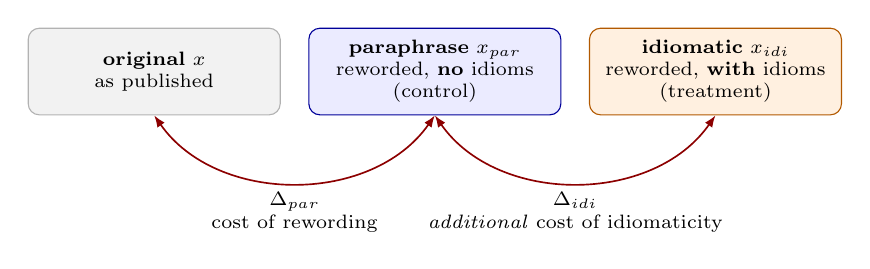
\begin{tikzpicture}[
      box/.style={rectangle, rounded corners, minimum width=3.2cm,
        minimum height=1.1cm, align=center, font=\scriptsize, inner sep=2pt},
      cmp/.style={{Latex[length=1.5mm]}-{Latex[length=1.5mm]}, semithick,
        draw=red!55!black}
    ]
    \node[box, draw=gray!60, fill=gray!10] (o) {\textbf{original} $x$\\ as published};
    \node[box, right=0.35cm of o, draw=blue!60!black, fill=blue!8] (p)
      {\textbf{paraphrase} $x_{\text{par}}$\\ reworded, \textbf{no} idioms\\ (control)};
    \node[box, right=0.35cm of p, draw=orange!70!black, fill=orange!12] (i)
      {\textbf{idiomatic} $x_{\text{idi}}$\\ reworded, \textbf{with} idioms\\ (treatment)};
    \draw[cmp] (o.south) to[out=-55,in=-125]
      node[midway, below, align=center, font=\scriptsize, text=black]
      {$\Delta_{\text{par}}$\\ cost of rewording} (p.south);
    \draw[cmp] (p.south) to[out=-55,in=-125]
      node[midway, below, align=center, font=\scriptsize, text=black]
      {$\Delta_{\text{idi}}$\\ \emph{additional} cost of idiomaticity} (i.south);
  \end{tikzpicture}\par}

  \vspace{0.2em}
  \[
    \Delta_{\text{par}} = \text{acc}_{\text{par}} - \text{acc}_{\text{orig}}
    \qquad
    \Delta_{\text{idi}} = \text{acc}_{\text{idi}} - \text{acc}_{\text{par}}
  \]
  \vspace{-0.3em}

  $\Delta_{\text{idi}}$ is measured against \textbf{paraphrase}, not original,
  so the rewording cost is subtracted out.
\end{frame}

% ---------------------------------------------------------------------
\begin{frame}{Why a Control Arm Is Necessary}
  \begin{itemize}
    \item Models are known to be sensitive to any semantics-preserving rewording
      (SEARs; Llama-2-70B-chat varying by 45.5 points between the best and worst
      of a set of semantically equivalent queries).
    \item A bare original-vs-idiomatic contrast confounds idiomaticity with
      generic paraphrase sensitivity.
    \item Prior idiom work measures \emph{comprehension} (detection tasks),
      not the downstream cost on a task not about idioms.
    \item Our design is a matched, semantics-preserving control arm over the
      \emph{same} items, not previously done for idiom-inserted NLU rewrites.
  \end{itemize}
\end{frame}

% ---------------------------------------------------------------------
\begin{frame}{Pipeline}
  \centering
  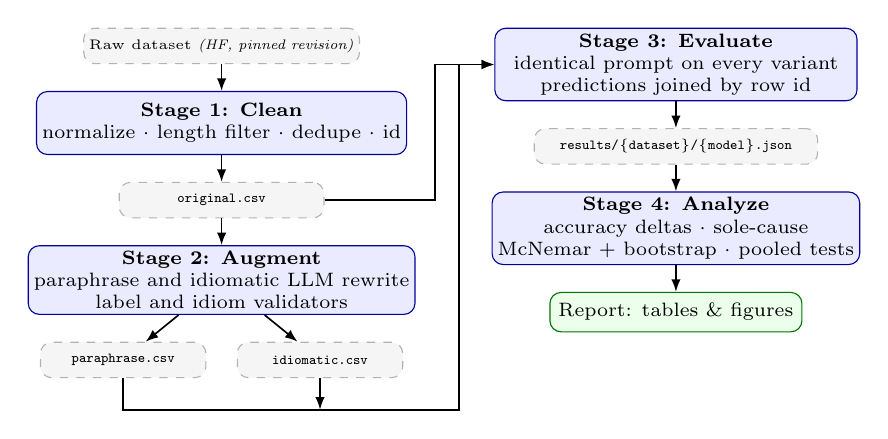
\begin{tikzpicture}[
      node distance=3.4mm,
      stage/.style={rectangle, rounded corners, draw=blue!60!black, fill=blue!8,
        minimum width=4.6cm, minimum height=0.8cm, align=center,
        font=\scriptsize, inner sep=2pt},
      artifact/.style={rectangle, rounded corners, draw=gray!60, fill=gray!8,
        dashed, minimum width=2.6cm, minimum height=0.45cm, align=center,
        font=\tiny, inner sep=2pt},
      finalbox/.style={rectangle, rounded corners, draw=green!45!black,
        fill=green!8, minimum width=3.2cm, minimum height=0.5cm, align=center,
        font=\scriptsize, inner sep=2pt},
      arrow/.style={-{Latex[length=1.6mm]}, semithick}
    ]
    % ---- left column: Stages 1-2 ----
    \node[artifact]               (raw)  {Raw dataset \textit{(HF, pinned revision)}};
    \node[stage, below=of raw]    (s1)   {\textbf{Stage 1: Clean}\\
                                          normalize $\cdot$ length filter $\cdot$ dedupe $\cdot$ id};
    \node[artifact, below=of s1]  (orig) {\texttt{original.csv}};
    \node[stage, below=of orig]   (s2)   {\textbf{Stage 2: Augment}\\
                                          paraphrase and idiomatic LLM rewrite\\
                                          label and idiom validators};
    \node[artifact, below=of s2, xshift=-1.25cm, minimum width=2.1cm] (para)
      {\texttt{paraphrase.csv}};
    \node[artifact, below=of s2, xshift=1.25cm, minimum width=2.1cm]  (idio)
      {\texttt{idiomatic.csv}};

    % ---- right column: Stages 3-4 ----
    \coordinate (colx) at ($(s2.east)+(1.0,0)$);
    \node[stage, anchor=north west] (s3) at (colx |- raw.north)
      {\textbf{Stage 3: Evaluate}\\ identical prompt on every variant\\
       predictions joined by row id};
    \node[artifact, below=of s3, minimum width=3.6cm] (res)
      {\texttt{results/\{dataset\}/\{model\}.json}};
    \node[stage, below=of res]  (s4)  {\textbf{Stage 4: Analyze}\\
                                       accuracy deltas $\cdot$ sole-cause\\
                                       McNemar + bootstrap $\cdot$ pooled tests};
    \node[finalbox, below=of s4] (rep) {Report: tables \& figures};

    \draw[arrow] (raw)  -- (s1);
    \draw[arrow] (s1)   -- (orig);
    \draw[arrow] (orig) -- (s2);
    \draw[arrow] (s2)   -- (para);
    \draw[arrow] (s2)   -- (idio);
    \draw[arrow] (s3)   -- (res);
    \draw[arrow] (res)  -- (s4);
    \draw[arrow] (s4)   -- (rep);

    % both rewritten variants feed Stage 3 up the gutter
    \coordinate (g)   at ($(s2.east)+(0.55,0)$);
    \coordinate (low) at ($(para.south)+(0,-0.4)$);
    \draw[arrow] (para.south) -- (para.south |- low) -- (idio.south |- low)
                 -- (g |- low) -- (g |- s3) -- (s3.west);
    \draw[arrow] (idio.south) -- (idio.south |- low);
    % original.csv bypasses Stage 2 and enters Stage 3 as the control variant
    \coordinate (g2) at ($(s2.east)+(0.25,0)$);
    \draw[arrow] (orig.east) -- (g2 |- orig) -- (g2 |- s3) -- (s3.west);
  \end{tikzpicture}

  \vspace{0.4em}
  {\scriptsize Four independently re-runnable stages, communicating only through
  versioned files on disk. \texttt{original.csv} feeds both Stage 2, as the
  rewriting source, and Stage 3, as the control variant.}
\end{frame}

% ---------------------------------------------------------------------
\begin{frame}{Datasets \& Models}
  \textbf{Three datasets}, one rewritten field each:
  \begin{itemize}
    \item \textbf{SST-2}: sentiment (sentence); \textbf{MMLU}: knowledge QA
      (question stem); \textbf{MNLI}: inference (premise)
    \item Aligned triples: 1{,}548, 1{,}085 and 4{,}709 rows
  \end{itemize}
  \vspace{0.5em}
  \textbf{14 instruction-tuned decoder LLMs}, 0.5B--7B, 10 families
  (Qwen2.5, Falcon3, OLMo-2, Gemma-2, Mistral, Phi-4-mini, Granite-3.1,
  H2O-Danube3, Yi-1.5, SmolLM2), zero-shot under an identical prompt per dataset.
  \vspace{0.5em}

  42 (model, dataset) runs, so 126 variant-level inference passes.
\end{frame}

% ---------------------------------------------------------------------
\begin{frame}{Statistical Framework}
  \textbf{Sole-cause test:} restrict to rows the model got right on
  \emph{original}, so any later error is caused by the rewrite, then count
  $b$ = idiomatic-only-wrong, $c$ = paraphrase-only-wrong. Rows where both
  rewrites agree carry no information and drop out.

  \vspace{0.3em}
  Tested two ways, required to \emph{agree}:
  \begin{itemize}
    \item \textbf{McNemar} $\chi^2$ with the Edwards continuity correction:
      \[
        \chi^2 = \frac{(|b - c| - 1)^2}{b + c}, \qquad \mathrm{df} = 1
      \]
      null: among discordant rows it is a coin flip which rewrite broke it.
    \item \textbf{Paired bootstrap}, 10{,}000 resamples of $b - c$, since the
      $\chi^2$ approximation is unreliable when $b + c$ is small.
  \end{itemize}
  Both agree in all 42 per-model runs. Also pooled per dataset (indicative, not
  a mixed-effects model).
\end{frame}

% ---------------------------------------------------------------------
\begin{frame}{Results: One Manipulation, Three Directions}
  \centering
  \begin{tabular}{lrrrl}
    \toprule
    Dataset & $n$ & $\Delta_{\text{par}}$ & $\Delta_{\text{idi}}$ & sig. ($-$/$+$) \\
    \midrule
    SST-2 & 1{,}548 & $-1.28$ & $\mathbf{+1.35}$ & 0/5 \\
    MMLU  & 1{,}085 & $+0.13$ & $-0.79$          & 1/0 \\
    MNLI  & 4{,}709 & $-0.68$ & $\mathbf{-1.28}$ & 10/0 \\
    \bottomrule
  \end{tabular}
  \vspace{1em}
  \raggedright

  \begin{itemize}
    \item \textbf{MNLI}: significant penalty for 10 of 14 models, and the
      sole-cause test agrees ($b > c$ for 12 of 14).
    \item \textbf{SST-2}: idioms \emph{help}, significant for 5 models and
      negative for none. One reading is that idioms here carry sentiment rather
      than obscure it, but nothing we ran isolates that.
    \item \textbf{MMLU}: marginal, surviving only in aggregate (1 of 14
      individually, $p = 0.0011$ pooled).
  \end{itemize}
  \vspace{0.2em}
  Idiomaticity is not a general accuracy tax: any account has to explain a
  change of \emph{sign} across tasks.
\end{frame}

% ---------------------------------------------------------------------
\begin{frame}{Every Model, Every Dataset}
  \centering
  \scriptsize
  \setlength{\tabcolsep}{3.5pt}
  \begin{tabular}{lrrr@{\hskip 1.2em}lrrr}
    \toprule
    Model & SST-2 & MMLU & MNLI & Model & SST-2 & MMLU & MNLI \\
    \midrule
    Qwen2.5-0.5B & $+0.45$ & $-1.75$ & $-0.40$ & Phi-4-mini-3.8B & $-0.19$ & $-1.84$ & $\bm{-1.51}^{\dagger}$ \\
    OLMo-2-1B & $+1.29$ & $-0.28$ & $\bm{-1.70}^{\dagger}$ & H2O-Danube3-4B & $\bm{+1.74}$ & $\bm{-2.49}$ & $+0.04$ \\
    Qwen2.5-1.5B & $+1.16$ & $-2.03^{\dagger}$ & $\bm{-1.59}^{\dagger}$ & Yi-1.5-6B & $+0.97$ & $-0.18$ & $\bm{-1.89}^{\dagger}$ \\
    SmolLM2-1.7B & $\bm{+2.20}$ & $-0.74$ & $+0.30$ & Qwen2.5-7B & $\bm{+3.04}^{\dagger}$ & $+0.09$ & $\bm{-1.17}^{\dagger}$ \\
    Gemma-2-2B & $+1.36^{\dagger}$ & $-1.38$ & $\bm{-1.51}^{\dagger}$ & Falcon3-7B & $-0.26$ & $+0.65$ & $\bm{-1.23}^{\dagger}$ \\
    Granite-3.1-2B & $\bm{+1.49}^{\dagger}$ & $+2.12$ & $-0.89$ & Mistral-7B-v0.3 & $\bm{+4.13}^{\dagger}$ & $-1.20$ & $\bm{-2.08}$ \\
    Falcon3-3B & $+0.39$ & $-0.37$ & $\bm{-2.25}^{\dagger}$ & OLMo-2-7B & $+1.16$ & $-1.66^{\dagger}$ & $\bm{-2.04}^{\dagger}$ \\
    \bottomrule
  \end{tabular}

  \vspace{0.2em}
  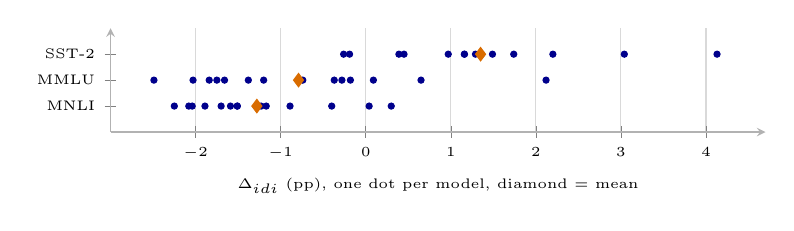
\begin{tikzpicture}
    \begin{axis}[
        width=9.9cm, height=2.9cm,
        symbolic y coords={MNLI, MMLU, SST-2}, ytick=data,
        xmin=-3.0, xmax=4.7, xtick={-2,-1,0,1,2,3,4},
        tick label style={font=\tiny},
        xlabel={$\Delta_{\text{idi}}$ (pp), one dot per model, diamond = mean},
        xlabel style={font=\tiny},
        axis lines=left, axis line style={gray!60},
        xmajorgrids, grid style={gray!30}, enlarge y limits=0.5,
      ]
      \addplot[only marks, mark=*, mark size=1.1pt, color=blue!55!black]
        coordinates {(0.45,SST-2) (1.29,SST-2) (1.16,SST-2) (2.20,SST-2)
          (1.36,SST-2) (1.49,SST-2) (0.39,SST-2) (-0.19,SST-2) (1.74,SST-2)
          (0.97,SST-2) (3.04,SST-2) (-0.26,SST-2) (4.13,SST-2) (1.16,SST-2)
          (-1.75,MMLU) (-0.28,MMLU) (-2.03,MMLU) (-0.74,MMLU) (-1.38,MMLU)
          (2.12,MMLU) (-0.37,MMLU) (-1.84,MMLU) (-2.49,MMLU) (-0.18,MMLU)
          (0.09,MMLU) (0.65,MMLU) (-1.20,MMLU) (-1.66,MMLU)
          (-0.40,MNLI) (-1.70,MNLI) (-1.59,MNLI) (0.30,MNLI) (-1.51,MNLI)
          (-0.89,MNLI) (-2.25,MNLI) (-1.51,MNLI) (0.04,MNLI) (-1.89,MNLI)
          (-1.17,MNLI) (-1.23,MNLI) (-2.08,MNLI) (-2.04,MNLI)};
      \addplot[only marks, mark=diamond*, mark size=2.4pt,
               color=orange!85!black]
        coordinates {(1.35,SST-2) (-0.79,MMLU) (-1.28,MNLI)};
    \end{axis}
  \end{tikzpicture}

  \vspace{-0.2em}
  \raggedright\scriptsize
  Ordered by parameter count. \textbf{Bold}: $\Delta_{\text{idi}}$ itself
  significant ($p<0.05$, McNemar exact). $\dagger$: the separate sole-cause $b$
  vs.\ $c$ gap is significant on \emph{both} tests. The two marks are
  independent, so a cell may carry either, both or neither.
\end{frame}

% ---------------------------------------------------------------------
\begin{frame}{Worked Disagreement Cases}
  \centering
  \scriptsize
  \setlength{\tabcolsep}{4pt}
  \begin{tabular}{@{}l p{6.3cm} l@{}}
    \toprule
    Variant & User prompt & Prediction \\
    \midrule
    \multicolumn{3}{@{}p{10.3cm}@{}}{\textbf{MNLI}, Falcon3-3B ($\Delta_{\text{idi}} = -2.25$~pp). Fixed hypothesis:
    \texttt{She now knows what was going on in her mind.} Gold: \emph{entailment}.} \\
    \addlinespace[1pt]
    original   & \texttt{Premise:} It took me really a long time to \textbf{sort} what was going on in my mind \textbf{out}, she said. & entailment $\checkmark$ \\
    paraphrase & \texttt{Premise:} She stated that it required a significant amount of time for her to \textbf{organize her thoughts}. & entailment $\checkmark$ \\
    idiomatic  & \texttt{Premise:} It took me quite a while to \textbf{wrap my head around} what was going on in my mind, she said. & contradiction $\times$ \\
    \midrule
    \multicolumn{3}{@{}p{10.3cm}@{}}{\textbf{SST-2}, Mistral-7B-v0.3 ($\Delta_{\text{idi}} = +4.13$~pp). Gold: \emph{positive}.} \\
    \addlinespace[1pt]
    original   & \texttt{Sentence:} is n't embarrassed to \textbf{make you reach for the tissues} & positive $\checkmark$ \\
    paraphrase & \texttt{Sentence:} is not ashamed to \textbf{make you cry} & negative $\times$ \\
    idiomatic  & \texttt{Sentence:} isn't shy about \textbf{pulling at your heartstrings} and making you reach for the tissues & positive $\checkmark$ \\
    \midrule
    \multicolumn{3}{@{}p{10.3cm}@{}}{\textbf{MMLU}, H2O-Danube3-4B ($\Delta_{\text{idi}} = -2.49$~pp). The four choices are
    untouched: \texttt{A.}\ a logical mistake.\ \texttt{B.}\ an ethical mistake.\
    \texttt{C.}\ a factual mistake.\ \texttt{D.}\ not a mistake. Gold: \emph{D}.} \\
    \addlinespace[1pt]
    original   & \texttt{Question:} \textbf{According to Nagel}, the view that moral luck is paradoxical is: & D $\checkmark$ \\
    paraphrase & \texttt{Question:} \textbf{Based on Nagel's analysis}, the perspective that moral luck is a paradox is: & D $\checkmark$ \\
    idiomatic  & \texttt{Question:} \textbf{In Nagel's eyes}, the view that moral luck is paradoxical is: & A $\times$ \\
    \bottomrule
  \end{tabular}

  \vspace{0.3em}
  \raggedright\scriptsize
  Each block is one row where a model with a \emph{significant}
  $\Delta_{\text{idi}}$ split between the two rewrites. \textbf{Bold} marks the
  aligned span; only the rewritten field changes within a block.
\end{frame}

% ---------------------------------------------------------------------
\begin{frame}{Key Insight: The Control Arm Changes the Story}
  \begin{columns}[T]
    \begin{column}{0.46\textwidth}
      \vspace{0.4em}
      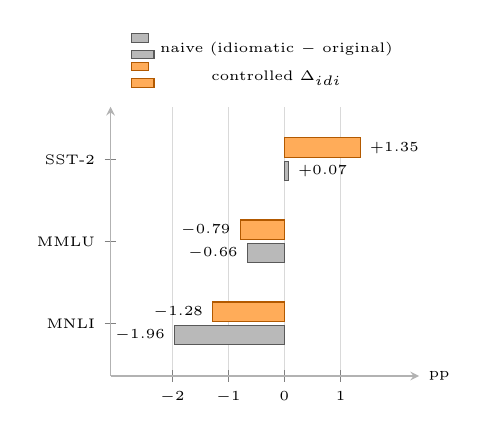
\begin{tikzpicture}
        \begin{axis}[
            width=5.5cm, height=5.0cm,
            xbar=1.5pt, bar width=7pt,
            symbolic y coords={MNLI, MMLU, SST-2}, ytick=data,
            xmin=-3.1, xmax=2.4,
            xlabel={pp}, xlabel style={font=\tiny, at={(1,0)}, anchor=west},
            tick label style={font=\tiny},
            legend style={font=\tiny, at={(0.5,1.04)}, anchor=south,
              legend columns=1, draw=none, fill=none},
            nodes near coords,
            nodes near coords style={font=\tiny, /pgf/number format/.cd,
              fixed, precision=2, print sign},
            xtick={-2,-1,0,1}, xmajorgrids, grid style={gray!30},
            axis lines=left, axis line style={gray!60},
            enlarge y limits=0.32,
          ]
          \addplot[fill=gray!55, draw=gray!70!black]
            coordinates {(0.07,SST-2) (-0.66,MMLU) (-1.96,MNLI)};
          \addplot[fill=orange!65, draw=orange!70!black]
            coordinates {(1.35,SST-2) (-0.79,MMLU) (-1.28,MNLI)};
          \legend{naive (idiomatic $-$ original),
                  controlled $\Delta_{\text{idi}}$}
        \end{axis}
      \end{tikzpicture}
    \end{column}
    \begin{column}{0.52\textwidth}
      \begin{itemize}
        \item Score idiomatic against \emph{original}, as a study without a
          control arm must, and SST-2 looks like a null ($+0.07$~pp) while
          MNLI's cost is overstated by roughly 53\%.
        \item The matched arm splits that false null into two real cancelling
          effects and cuts MNLI's to its idiom-specific size. Neither
          correction is visible without it.
        \item The magnitudes are real but modest: a 1--2~pp MNLI drop is the
          same order as plain rewording's own cost, not an order above it.
        \item So idiomaticity is one \textbf{distinguishable contributor} to
          paraphrase sensitivity, not a separate failure mode.
      \end{itemize}
    \end{column}
  \end{columns}
\end{frame}

% ---------------------------------------------------------------------
\begin{frame}{Scale Does Not Explain It}
  \begin{columns}[T]
    \begin{column}{0.45\textwidth}
      \vspace{0.6em}
      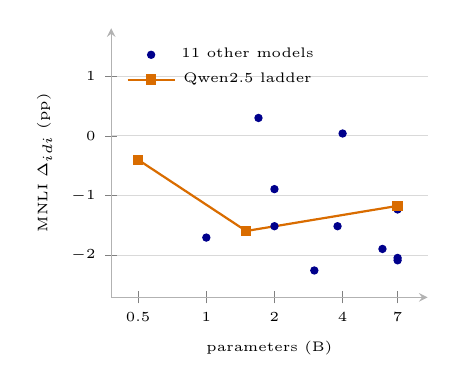
\begin{tikzpicture}
        \begin{axis}[
            width=5.6cm, height=5.0cm,
            xmode=log, log basis x=10,
            xtick={0.5,1,2,4,7}, xticklabels={0.5,1,2,4,7},
            xlabel={parameters (B)},
            ylabel={MNLI $\Delta_{\text{idi}}$ (pp)},
            label style={font=\tiny}, tick label style={font=\tiny},
            xmin=0.38, xmax=9.5, ymin=-2.7, ymax=1.8,
            ytick={-2,-1,0,1}, ymajorgrids, grid style={gray!30},
            axis lines=left, axis line style={gray!60},
            legend style={font=\tiny, at={(0.02,0.97)}, anchor=north west,
              draw=none, fill=none},
          ]
          \addplot[only marks, mark=*, mark size=1.3pt, color=blue!55!black]
            coordinates {(1,-1.70) (1.7,0.30) (2,-1.51) (2,-0.89) (3,-2.25)
                         (3.8,-1.51) (4,0.04) (6,-1.89) (7,-1.23) (7,-2.08)
                         (7,-2.04)};
          \addplot[mark=square*, mark size=1.5pt, color=orange!85!black, thick]
            coordinates {(0.5,-0.40) (1.5,-1.59) (7,-1.17)};
          \legend{11 other models, Qwen2.5 ladder}
        \end{axis}
      \end{tikzpicture}
    \end{column}
    \begin{column}{0.53\textwidth}
      \begin{itemize}
        \item $\Delta_{\text{idi}}$ correlates with neither original accuracy
          nor parameter count ($p > 0.3$ on all three datasets).
        \item The Qwen2.5 ladder shows it concretely: MNLI's penalty is
          non-monotone at $-0.40$, $-1.59$, $-1.17$~pp across 0.5B, 1.5B and 7B,
          and all four 7B models sit inside the degraded group.
        \item With 14 models, $|\rho|$ must reach about $0.53$ before the test
          can call anything significant: absence of evidence, not evidence of
          absence.
        \item Takeaway: \textbf{nothing here supports waiting for a larger
          checkpoint}, and settling the question needs many more models than 14.
      \end{itemize}
    \end{column}
  \end{columns}
\end{frame}

% ---------------------------------------------------------------------
\begin{frame}{Limitations}
  \begin{itemize}
    \item Parse-failure filtering is blunt and non-random (up to 12.4\% dropped
      for one model/dataset pair).
    \item Pooled tests treat repeated rows as independent, giving optimistic p-values.
    \item No multiple-comparisons correction; no mixed-effects re-analysis.
    \item Zero-shot, greedy decoding, single prompt template, decoder-only panel.
  \end{itemize}
\end{frame}

% ---------------------------------------------------------------------
\begin{frame}{Future Work}
  \begin{itemize}
    \item Verify rewrites preserve meaning; run a mixed-effects re-analysis of
      the pooled claims.
    \item Score idiom \emph{opacity} and \emph{frequency} against
      $\Delta_{\text{idi}}$. Both reuse the rewritten text already collected,
      but Stage 2 recorded no inventory of which idiom it inserted, so each
      row's idiom must be identified first.
    \item Rewrite MNLI's hypothesis or MMLU's answer choices too, making idiom
      position a manipulated variable \emph{within} one dataset.
    \item Try to \emph{reduce} the penalty: few-shot prompting, and brief
      fine-tuning to test whether it is a fixable exposure gap.
  \end{itemize}
\end{frame}

% ---------------------------------------------------------------------
\begin{frame}{Summary}
  \begin{itemize}
    \item We measured the accuracy cost of idiomatic phrasing for 14
      instruction-tuned decoder LLMs (0.5B--7B) on SST-2, MMLU and MNLI, pairing
      every idiomatic rewrite with a matched non-idiomatic paraphrase of the
      same row, so the cost of rewording is subtracted rather than absorbed.
    \item That control is what makes the result readable: without it SST-2 looks
      like a null and MNLI's idiom-specific penalty is overstated by roughly
      53\%.
    \item With it the penalty concentrates on \textbf{MNLI}: $-1.28$~pp,
      significant for 10 of the 14 models, against $-0.79$~pp on MMLU with a
      single significant model and no penalty at all on binary sentiment. These
      are means across models, not pooled figures.
    \item Idiomaticity is therefore a distinguishable contributor to paraphrase
      sensitivity rather than a separate failure mode. No scale trend is
      detectable across a 14-fold parameter range, though a panel of 14 models
      could not have detected a moderate one.
  \end{itemize}
\end{frame}

\begin{frame}
  \centering
  \Huge Thank you\\[0.5em]
  \Large Questions?
\end{frame}

\end{document}
